\documentclass[11pt,letterpaper]{article}
\usepackage[T1]{fontenc}
\usepackage{lmodern,amsmath,amssymb,graphicx,xcolor,booktabs,microtype}
\usepackage[margin=.9in,top=.83in,bottom=.88in,headheight=14pt]{geometry}
\usepackage{fancyhdr,enumitem,titlesec}
\usepackage[colorlinks=true,allcolors=teal!63!black]{hyperref}
\definecolor{ink}{HTML}{183747}
\definecolor{tealink}{HTML}{126F70}
\definecolor{paperblue}{HTML}{EAF3F1}
\titleformat{\section}{\sffamily\Large\bfseries\color{ink}}{\thesection}{.65em}{}
\setlength{\parindent}{0pt}\setlength{\parskip}{4.5pt plus 1pt}
\setlist{itemsep=2pt,topsep=4pt}
\setlength{\emergencystretch}{1.5em}
\pagestyle{fancy}\fancyhf{}
\fancyhead[L]{\sffamily\small\color{ink}Universal convex covers of space curves}
\fancyfoot[R]{\sffamily\small\color{ink}\thepage}
\renewcommand{\headrulewidth}{.3pt}
\hypersetup{pdftitle={How small a convex body covers every unit space curve?},pdfauthor={Research note for Vladimir Reshetnikov}}
\newcommand{\RR}{\mathbb R}\DeclareMathOperator{\vol}{vol}
\newcommand{\lowerresult}{0.018975}
\begin{document}
\thispagestyle{plain}
{\sffamily\color{tealink}\small CONVEX GEOMETRY\hfill 19 NOVEMBER 2026\par}
\vspace{9pt}
{\sffamily\bfseries\color{ink}\fontsize{26}{30}\selectfont How small a convex body covers\\ every unit space curve?\par}
\vspace{5pt}
Let $V_3$ be the least volume of a compact convex body in $\RR^3$ that can contain every smooth unit-length curve after a rotation and a translation chosen for that curve. Endpoints are free. The following bounds improve both estimates in the supplied reports.
\begin{center}
\setlength{\fboxsep}{9pt}\colorbox{paperblue}{\makebox[.80\linewidth]{\large $\displaystyle \lowerresult < V_3 < 0.052956040$}}
\end{center}
The upper bound is the volume bound for an explicit convex body. The lower bound uses four compulsory objects, including a space curve whose convex hull contains a ball. A minimizing body exists. The shape of a minimizer and a closed-form evaluation of $V_3$ remain open here. Section~4 gives $V_3$ as a convergent series of finite rational calculations, with an explicit remainder bound.
\begin{center}
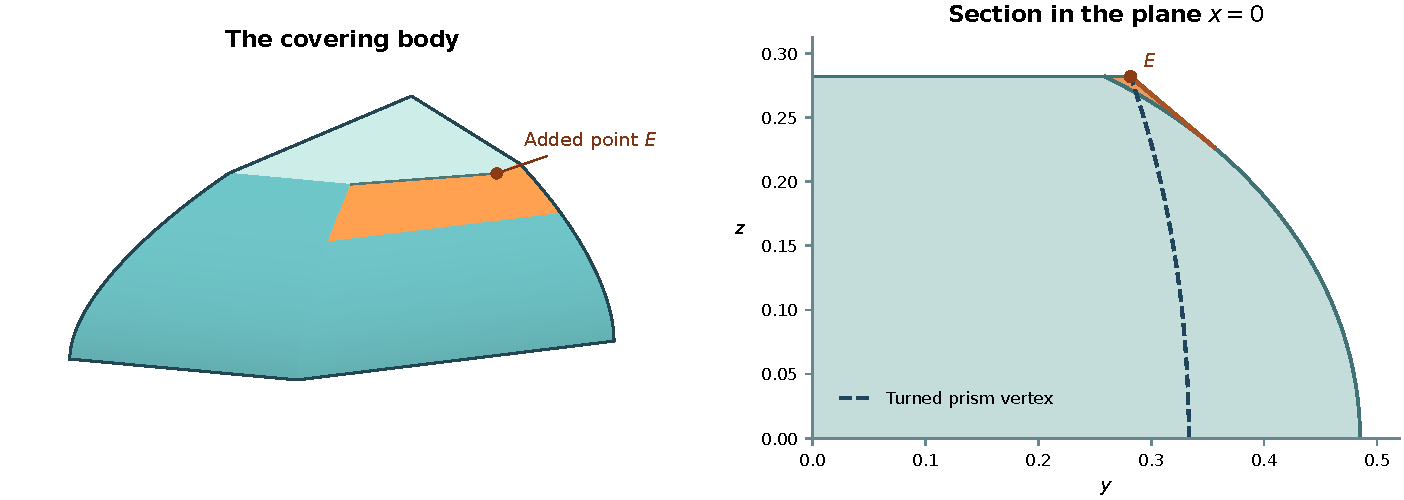
\includegraphics[width=.96\linewidth]{figures/construction.pdf}
\end{center}
{\small\sffamily\color{ink}The extra point $E$ allows the tall enclosing prisms to lie on their sides. Only one of the original four curved side faces contributes extra volume.}
\medskip
\begin{center}
\begin{tabular}{@{}lrr@{}}
\toprule
&Lower bound&Upper bound\\\midrule
First report, \texttt{space\_worm} & $0.0187328127\ldots$ & $0.0542670928\ldots$\\
Second report, published inputs & $3/220$ & $\pi/54$\\
Second report, with Keller's quadrilateral & $3/220$ & $0.0547404972\ldots$\\
This paper, certified decimals & $\lowerresult$ & $0.052956040$\\\bottomrule
\end{tabular}
\end{center}
\clearpage
\section{Curves, compactness, and the two earlier bounds}
A curve is an ordered path, with retracing counted in its length. Containment concerns its image, including its endpoints. A rigid motion here has the form $x\mapsto Rx+t$ with $R\in SO(3)$. All upper-bound placements use proper rotations. Length $L>0$ multiplies the answer by $L^3$, by dilating the curves and the container.
\paragraph{Why smooth curves force the polygonal tests.}
Every rectifiable unit path can be approximated uniformly, up to reparametrization, by regular smooth paths of length exactly one. Here are details relevant to the lower bounds. Take inscribed polygonal paths whose meshes tend to zero and whose lengths tend to one. Perturb their vertices by amounts small enough to preserve both limits and to make all chords nonzero and consecutive chords nonopposite. Parametrize each polygon by arclength and continue its first and last edges linearly just beyond the endpoints. Convolve with a nonnegative smooth kernel of integral one supported on an interval shorter than half the smallest edge length. Near a corner the derivative is a convex combination of its two adjacent unit tangents, hence never zero. Elsewhere the derivative is the original tangent. As the kernel support tends to zero, both the positions and the lengths converge to those of the polygon. Dilating each smoothed arc about its start to give it length exactly one preserves convergence. If one also requires simple curves, choose the perturbed polygon in general position in three dimensions so that nonadjacent edges are disjoint, and round the corners inside disjoint balls.
For each approximant anchored at the origin, a fitting motion has its translation in the compact container and its rotation in the compact group $SO(3)$. A convergent subsequence of motions therefore places the original path in the closed container. A shorter path can first be extended to length one. This also explains why closing the two endpoints is an additional restriction on the problem.
\paragraph{Attainment.}
Let $T$ be the tetrahedron with successive vertices $0$, $e_1/3$, $(e_1+e_2)/3$, and $(e_1+e_2+e_3)/3$, where the $e_i$ are the coordinate unit vectors. Its three-edge path has length one. A universal body contains a copy of $T$, hence a fixed positive-radius ball after a rigid motion. Write its radius as $r$ and fix its center $o$. For any $x$ in the body, the cone from $x$ to the radius-$r$ disk through $o$ perpendicular to $x-o$ has volume $\pi r^2\|x-o\|/3$. Thus any minimizing sequence of bounded volumes, normalized around this ball, lies in a common bounded region. The radius-$1/2$ ball is already universal, since the arclength midpoint is within distance $1/2$ of the entire path.
By Blaschke selection a subsequence has a Hausdorff limit $K_*$. Volume converges, for a Hausdorff error $\delta$ puts either body inside the other's dilation about $o$ by $1+\delta/r$. For each fixed curve a further subsequence of its rigid placements converges and places it in $K_*$. Thus $K_*$ is universal and attains the infimum.
\paragraph{What changes from the supplied reports.}
H\aa stad, Linusson and W\"astlund studied this spatial covering problem in \cite{hlw}. Both reports reduce a spatial curve to a right prism using alternating support planes. The second keeps the entire family of heights, giving a volume factor $2/9$ times the area of a planar cover. With the published sector of \cite{sector}, the upper bound is $\pi/54$. Its four-link lower witness has minimum projected area $9/220$, which gives its lower bound $3/220$ by the fiber inequality below. The first cuts the family at height $4/13$ and uses a segment and two width tests to obtain its stronger interval. Here the quadrilateral's actual side directions allow a lower cut, and a fourth test constrains the surface area of every admissible body.
\clearpage
\section{Turning the entire enclosing prism}
The base is Keller's planar universal quadrilateral $C$ \cite[Theorem 4.1]{keller}. For $n(t)=(1-t^2,2t)/(1+t^2)$, its definition is
\[
 C=\{v\in\mathbb R^2:n(t_i)\cdot v\le d_i,\quad 0\le i\le3\},\qquad
 \begin{array}{c|rrrr}
 i&0&1&2&3\\ \hline
 t_i&-631/58&-1&7/16&37/56\\
 d_i&0&0&130783/250000&446199/10^6
 \end{array}
\]
 Index its four support lines cyclically from
$0$ through $3$, and write $n_i=(a_i,b_i)$ and $d_i$ for their unit
normals and offsets. The origin
is a vertex. Denote the intersection of lines $j$ and $j+1$ by $(x_j,y_j)$,
using indices modulo four. Write $x_* = x_3=\min_jx_j$ and
$Y=y_3=\max_j y_j$. The two bottom vertices have $y_0=y_1=0$.
Set
\[
 T=1/Y,\qquad H=(9+T^2)^{-1/2}=0.281666408810\ldots.
\]
Begin with the tapered body
\[
 K_0=\{(x,y,z):0\le z\le H,\quad(x,y)\in\sqrt{1-9z^2}\,C\}.
\]
The scale is nonnegative and concave on $[0,H]$. Since $0\in C$,
its scaled copies are nested, so $K_0$ is convex. Add one point $E=(0,H,H)$ and take $K=\operatorname{conv}(K_0\cup\{E\})$.

For a nonplanar curve choose the normal to the alternating support planes of Ghomi \cite[Corollary 3.2]{ghomi}, put $h$ equal to their separation, and write
$p=\sqrt{1-9h^2}$. The curve meets one plane, then the other, then the first and then the other again. Each of the three intervening portions contributes at least $h$ to the total variation of the vertical coordinate. The triangle inequality for the integrated horizontal and absolute
vertical speeds bounds the projected length by $p$. Indeed, in arclength coordinates,
\[
  L_{xy}^2+\operatorname{TV}(z)^2=
  \left\|\int_0^1 (\|\gamma'_{xy}\|,|z'|)\,ds\right\|^2\le1 .
\] A planar curve can
be treated with $h=0$. By Keller's covering theorem and scaling, the whole
spatial curve fits a right prism with base $p C$ and height $h$. If the
planar placement uses a reflection, also reverse the vertical coordinate
and translate its range to $[0,h]$. This gives a proper spatial motion.
For $h\le H$, this prism fits directly at the bottom of $K_0$.

For $H\le h\le1/3$, turn the prism through a right angle and translate it.
Its image can be written
\[
 Q_h=\{(p(x-x_*),s,py):(x,y)\in C,\quad 0\le s\le h\}.
\]
For example, the rotation $(x,y,z)\mapsto(x,-z,y)$ followed by translations
gives the displayed set. Only the eight vertices need to be tested because
$K$ is convex. Put $t=p/h$, so $0\le t\le T$. Since $TY=1$ and $p$
decreases with $h$, the largest height $pY$ occurs at $H$ and is at
most $HTY\le H$. Both horizontal coordinates of $Q_h$ are nonnegative.
Thus the first two inequalities of the horizontal sections hold.
The remaining normals have positive coordinates, so only $s=h$ can be
extremal. For $i=2,3$ and $X_j=x_j-x_*$ the required inequalities are
\[
 a_i p X_j+b_i h\le d_i\sqrt{1-9p^2 y_j^2}.
\]
Squaring, dividing by $h^2$, and using $h^{-2}=9+t^2$ gives the test
$A t^2+B t+D\le0$, where
\[
 A=(a_i X_j)^2+9d_i^2y_j^2-d_i^2,\quad B=2a_iX_j b_i,\quad
 D=b_i^2-9d_i^2.
\]
For seven entries rational upper bounds for the maximum over $[0,1/Y]$
are given below. One evaluates the polynomial at $0$, at $1/Y$, and at
$-B/(2A)$ when $A<0$ and this last point belongs to the interval.
\[
\begin{array}{c|rrrr}
 &j=0&j=1&j=2&j=3\\\hline
 i=2&-1.91&-0.014&-0.60&-0.44\\
 i=3&-0.93&-0.055&-0.18&\text{extra point}
\end{array}
\]
Only the vertex $(0,h,pY)$ can escape $K_0$. Let $m=d_3/b_3$.
Then $(0,m,0)\in K_0$. At every height $0\le z\le H$ the point $(0,0,z)$
lies in $K_0$, and the segment from $(0,m,0)$ to $E$ lies in $K$.
The resulting allowable interval of $y$ at $x=0$ reaches
$m-(m-H)z/H$. Along the exceptional vertex locus,
$y=g(z)=\sqrt{1-z^2/Y^2}/3$, for $0\le z\le H$.
Here $g(H)=H$ and $|g'(z)|\le |g'(H)|=1/(9Y^2)\le(m-H)/H$.
The available interval contains this vertex as well.

The addition of $E$ changes just one curved face of $K_0$.
Indeed, $E$ satisfies the defining inequalities of the bottom, top and
first three side surfaces viewed separately. Each such inequality defines
a convex set, so none of its supporting planes has $E$ strictly outside.
Let $e$ be the base edge between vertices 2 and 3, $L$ its length,
$s(z)=\sqrt{1-9z^2}$, $b=b_3$ and $d=d_3$.
The volume added by $E$ is the integral of its positive signed distance to
the supporting plane, times surface area divided by three, over the fourth
face. This cone formula follows by joining each visible surface element to
$E$. Equivalently, the parametrization $(r,u)\mapsto E+r(u-E)$ of the added
region, with $0\le r\le1$ and visible boundary point $u$, has volume
element $r^2(E-u)\cdot n(u)\,dr\,dS(u)$, where $n(u)$ is the outward
unit normal. Shared boundary pieces have volume zero.

At height $z$ the edge has length $L s(z)$ and the outward normal is
proportional to $(n_3,-d s'(z))$. Normalization cancels the area
factor $\sqrt{1+d^2s'(z)^2}$. For $u$ on this edge,
the resulting integrand before dividing by three is
$L s(z)[bH-ds(z)-ds'(z)(H-z)]_+$.
The identity $s(z)^2+s(z)s'(z)(H-z)=1-9Hz$ yields
\[
 |K|=|C| H(1-3H^2)
  +\frac L3\int_0^H
  \left[bH\sqrt{1-9z^2}-d(1-9Hz)\right]_+\,dz
  =0.05295603908\ldots .
\]
This integral also has an elementary closed form. With $c=bH/d$, let $z_0$ be the root in $(0,H)$ of
$(81H^2+9c^2)z_0^2-18Hz_0+1-c^2=0$. The expression inside the positive part is strictly concave, negative at zero and positive at $H$. Its positive interval is therefore $(z_0,H]$. An antiderivative there is
\[
 F(z)=bH\left(\tfrac z2\sqrt{1-9z^2}+\tfrac16\arcsin(3z)\right)-d\left(z-\tfrac92 Hz^2\right).
\]
The volume correction is exactly $L(F(H)-F(z_0))/3$.

For a rational evaluation put $z=Hv$. The expression inside the positive part becomes
$g(v)=bH\sqrt{1-9H^2v^2}-d(1-9H^2v)$.
It is concave, with $|g''|=9bH^3(1-9H^2v^2)^{-3/2}<3$ throughout $[0,1]$, using $1-9H^2>1/4$. Divide $[0,1]$ into $8192$ equal intervals. On each one $g$ exceeds its chord by at most $3/(8\cdot8192^2)$, by the linear interpolation error bound. Taking positive parts preserves that error. The integral of the positive part of a chord is the area of a trapezoid or a triangle. The verifier rounds each square root down to a multiple of $10^{-15}$ for these chords and adds the rounding and interpolation errors to the upper integral. It obtains the rigorous enclosure
\[
        0.0529560390 < \vol(K) < 0.052956040 .
\]

\clearpage
% Self-contained section; requires amsmath.
\section{A larger lower bound}
Write $V$ for the volume of any universal body $K$. Three witnesses force
a unit segment in $K$, a planar curve of planar width greater than
$b=0.43892$, and a space curve of width greater than $w=0.25607$.
These are respectively the segment, the rescaled Adhikari--Pitman caliper,
and the rescaled Bartels--Choy--Wu--Li curve as in the original report.
A fourth witness forces a ball. For the strongest endpoint below, take $r=1/9.577$. Zalgaller's open inspection curve has length to hull-inradius ratio below $9.577$ \cite[p.~125, following Theorem~1.2]{ghomi}. Enclosing the curve encloses its convex hull. An independent rational polygon in the accompanying code gives $r=0.1043499$ and a lower bound within $0.000005$ of the stronger one. The two widths follow from the respective width-one lengths $<2.27830$ and $<3.90513$ \cite{ap,bartels}. Each witness is free to occupy its own position.

Project $K$ perpendicular to its unit segment, onto a planar body $P$
of area $A$, perimeter $p$, and diameter $d$. We have $d\ge b$ and
every width of $P$ is at least $w$. Indeed the plane of the caliper contains
some direction parallel to the projection plane, and the spatial width
bound holds in all directions. To see $3V\ge A$, observe that fibers parallel to the
unit segment have length at least $t$ on a $(1-t)$-scaled copy of $P$,
by taking convex combinations with the segment. Integrating their superlevel areas gives $V\ge A\int_0^1(1-t)^2\,dt=A/3$.

Let $S$ denote the surface area of $K$ and $m$ its unit outer normal,
defined almost everywhere. Write $m_u,m_H$ for its component along
the unit segment and its horizontal projection. The projection area
formula gives $\int|m_u|\,dS=2A$. For a horizontal unit normal $e$, the
projection of $K$ onto $e^\perp$ contains the unit segment and has transverse
span $W_P(v)$, where $v$ is the horizontal unit vector perpendicular to $e$.
Taking the two triangles on the segment gives projected area at least
$W_P(v)/2$. Integrate over $e$ on the horizontal unit circle.
The projection formula and $\int|m_H\cdot e|\,de=4|m_H|$ give
$2\int|m_H|\,dS\ge p$, using $\int W_P(v)\,dv=2p$.
The triangle inequality for integrals now gives
$S\ge\sqrt{(p/2)^2+(2A)^2}$. Since $K$ contains an $r$-ball,
the divergence theorem about its center gives $3V\ge rS$
(equivalently, sum the volumes of the pyramids over the facets and
take a polyhedral limit).


Choose a diameter of $P$ as base from $O=(0,0)$ to $B=(d,0)$. Every point has first coordinate in $[0,d]$. Take a highest and a lowest point $C=(x,h)$ and $F=(y,-k)$ and let $H=h+k$. The quadrilateral $Q=\operatorname{conv}\{O,B,C,F\}$ has area $dH/2$. Thus $2A\ge dH\ge bw$. The perimeter $p$ bounds the length of the quadrilateral's two broken paths $OCB$ and $OFB$. By reflecting across each horizontal extremal line, their lengths are at least $\sqrt{d^2+4h^2}$ and $\sqrt{d^2+4k^2}$, respectively.
\begin{center}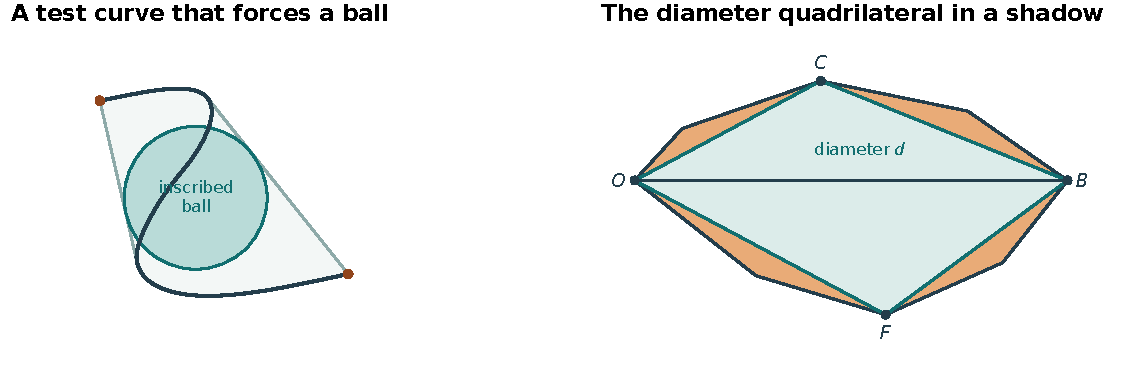
\includegraphics[width=.92\linewidth]{figures/lower_geometry.pdf}\end{center}
{\small\sffamily\color{ink}Left, the independent 61-vertex test curve and the orthogonal shadow of its inscribed ball. Right, the excess area is the sum of the four orange regions between the shadow boundary and the quadrilateral.}
\paragraph{How the two oblique widths use the excess area.}
Retain the notation $A,d,H,h,k,x,y$ of the diameter quadrilateral.
Reflect vertically if necessary so that $0\le h\le k$ and write $f=h/H$.
Set $E=A-dH/2$. The surface and the two reflected polygonal paths imply
\begin{equation}
 (3V)^2\ \ge\ r^2\left[
 \tfrac14\left(\sqrt{d^2+4H^2 f^2}
       +\sqrt{d^2+4H^2(1-f)^2}\right)^2+d^2H^2\right].
 \label{eq:edge-surface}
\end{equation}
In fact $S\ge\sqrt{(p/2)^2+(2A)^2}$, $3V\ge rS$, and $2A\ge dH$.

For the upper supporting vertex $C=(x,h)$, define $e_{ul}$ and $e_{ur}$
as the areas of the portions of $P$ beyond the lines $OC$ and $CB$,
on the side away from triangle $OCB$. Define $e_{bl},e_{br}$ in the
reflected lower half analogously, using $F=(y,-k)$. These four portions
have disjoint interiors and total area $E$. Indeed, on the upper half the
two outside tests have left sides
\[
  U=xY-hX,\qquad T=h(X-x)+(d-x)(Y-h)
\]
at a point $(X,Y)$. Their sum is $d(Y-h)\le0$, and neither is positive on
the lower half. If $T>0$, the triangle with the point and the edge $CB$
lies in the upper-right portion, so $T\le2e_{ur}$. The same argument
gives $U\le2e_{ul}$, with corresponding formulas below.

Assume first $h>0$ and take
\[
 a_+=\max\{(d-x)/h,\ y/k\},\qquad
 a_-=\max\{x/h,\ (d-y)/k\}.
\]
The maximum of $X+a_+Y$ exceeds $x+a_+h$ by at most $2e_{ur}/h$.
This follows from
\[
   X-x+a_+(Y-h)=T/h+\bigl(a_+-(d-x)/h\bigr)(Y-h).
\]
Its minimum is at least $y-a_+k-2e_{bl}/k$ by the reflected
lower-left inequality. Its width is at least $w\sqrt{1+a_+^2}$. Applying
the same argument to $-X+a_-Y$ uses the two remaining edge areas.
On addition the horizontal offsets $x-y$ cancel, giving, with
$s=a_++a_-$,
\[
   w\sqrt{4+s^2}\ \le\ w\bigl(\sqrt{1+a_+^2}+\sqrt{1+a_-^2}\bigr)
    \ \le\ Hs+2E/h .
\]

Here $k\ge h$. For $D_*=hs$, the last inequality becomes
\[
 w(\sqrt{D_*^2+4h^2}-D_*)\le 2A-dw+(H-w)(D_*-d).
\]
The left side decreases with $D_*$, while the right side increases. Upper bounds on $D_*$ will suffice.

Put $t=h/k$, $X_0=|x-d/2|$ and $Y_0=|y-d/2|$. Expand the two maxima defining $s$. After multiplying by $h$, their possible sums are $d$, $dt$, $x+ty$, and $(d-x)+t(d-y)$. Consequently
\[
 d\le D_*\le d+\Delta,\qquad
 \Delta=\min\{dt,\max(0,-d(1-t)/2+X_0+tY_0)\}.
\]
Suppose now that $3V\le A_0$. The surface inequality gives $p\le p_{\max}=2\sqrt{(A_0/r)^2-d^2H^2}$. The upper broken path $OCB$ has length at most $\ell=p_{\max}-\sqrt{d^2+4k^2}$. Thus $C$ belongs to the ellipse of foci $O,B$ and major axis $\ell$. From its equation,
\[
 X_0\le\min\left\{d/2,\frac{\ell}{2}\sqrt{1-\frac{4h^2}{\ell^2-d^2}}\right\}.
\]
The case $\ell<\sqrt{d^2+4h^2}$ immediately contradicts the upper path's length. Interchanging $h,k$ bounds $Y_0$ as well. If $h=0$, the perimeter test alone applies.

\paragraph{The finite check.}
For $A_0=3(0.018975)$, the only possible parameter box is
\[
 b\le d\le2A_0/w,\quad w\le H\le2A_0/b,\quad 0\le f=h/H\le1/2.
\]
The included checker bisects it into 24 boxes. In each box the sum of the two square roots in \eqref{eq:edge-surface} is bounded below using the lower endpoints for $d,H$ and the upper endpoint for $f$, since that sum decreases as $f$ increases to $1/2$. The area bound $dH\le2A_0$ tightens both upper endpoints. For each ellipse, an upper bound on $\ell$ and lower bounds on its own height and the focal distance give upper bounds on the two offsets. The checker substitutes an upper bound for $D_*$ and a lower bound for $h$ in the decreasing left side of the oblique-width test, and upper bounds for $A,H,\Delta$ and a lower bound for $d$ on its right. When a box still overlaps $h=0$, the offset bound $d/2$ suffices. In the zero-height case the oblique-width test reduces to $0\le2A-dw$, so a width exclusion cannot accidentally discard a feasible zero-height case.
All arithmetic is rational with outward rounding of square roots at precision $10^{-12}$. Seventeen boxes fail the surface or ellipse test and seven fail the width test. This proves $V>0.018975$.

Using the explicit polygon in \texttt{check\_inspection.py} gives $V>0.01897$ by the identical 23-bisection calculation with $r=0.1043499$. Its 61 vertices are integer triples in units of $10^{-7}$. Rounding each integer link length upwards bounds the path length by $0.9999834$. Every facet plane contains a noncollinear triple. The checker enumerates all triples and tests every supporting plane $n\cdot X=c$ in integer coordinates, oriented outwards. It finds $c>0$ and $c^2\ge(1043499)^2\|n\|^2$ for every supporting triple, proving ball containment.

\section{An exact series for the volume}

The value can be specified without any optimization over real parameters. The series below uses finite integer and rational operations for each term. The large catalogues make it expensive to evaluate.

For each positive integer $n$, take mesh size $n^{-3}$ and form all
$n$-step walks starting at the origin with increments
\[
    d=n^{-3}(i,j,k),\qquad i^2+j^2+k^2\le n^4,\qquad i,j,k\in\mathbb Z.
\]
Each walk has length at most one. Use the same fixed tetrahedron $T$ as in Section~1. In the
coordinates $0\le z\le y\le x\le1/3$, its four facet planes are explicit.
The closed ball of radius $r=1/15$ around
$o=(4/15,1/6,1/15)$ lies in $T$. The distances to the two sloping facets are
$1/(10\sqrt2)>1/15$.

Here is a finite catalogue of poses. Set $m=n^2$. Choose an integer
quaternion $q$ by setting one of its four components equal to $m$ and
letting each other component run from $-m$ to $m$. Let $R_q$ be its
rotation, defined on vectors viewed as pure quaternions by
$R_q(v)=qv\overline q/\|q\|^2$. Use all maps
\[
     v\longmapsto R_qSv+t,\qquad
     t\in m^{-1}\mathbb Z^3\cap[-114,114]^3,
\]
where $S$ ranges over the $24$ orientation-preserving signed permutations
of the coordinates. The extra signed permutations make the order-one
example shorter. All entries of the maps are rational. Choose one pose
independently for every walk. Let $b_n$ be the least volume of the convex
hull of $T$ and all the resulting vertices, over this finite list of
choices.

For clarity, a finite arithmetic specification of this coefficient is
as follows. Enumerate all tuples of pose indices, one index per walk.
For each tuple, make its list of points and enumerate all noncollinear
triples. Keep the triples whose plane has every point on one closed side.
Merge triples with the same supporting plane and order its extreme points
cyclically using a projection onto a nondegenerate coordinate plane and
a planar convex hull. Triangulate each resulting face from one of its
vertices. For each boundary triangle $a,b,c$ add
$|\det(a-g,b-g,c-g)|/6$, where $g$ is the average of all the distinct
points. Since $T$ is full-dimensional, $g$ is interior, and these pyramids
decompose the hull in volume. Take the least sum found. Thus $b_n$ is
obtained from integers by finite rational arithmetic and comparisons.

Define the rational numbers
\[
   d_n=\frac1{2n}+\frac7{4n^2},\qquad
   e_n=\frac9{2n^2},\qquad
   L_n=\frac{b_n}{(1+15e_n)^3},\qquad
   U_n=b_n(1+15d_n)^3.
\]
Then $L_n\le V_3\le U_n$. In particular, if
$c_j=\max_{0\le k\le j}L_{2^k}$, then
\[
  \boxed{\displaystyle V_3=c_0+\sum_{j=0}^{\infty}(c_{j+1}-c_j).}
\]
All summands are nonnegative. After summing through $c_j$, with $n=2^j$,
the uncomputed tail is bounded both by $U_n-c_j$ and by
\[
 45(0.052956040)\left(\frac1{2n}+\frac{25}{4n^2}\right).
\]

\paragraph{Proof of the upper estimate.}
Parametrize a unit curve by arclength and place its first point at the
origin. Divide the parameter interval into $n$ equal pieces. Round each
coordinate of each endpoint increment towards zero on the $n^{-3}$
mesh. This shortens each increment, so the resulting walk occurs in our
finite family. A rounded sample point is within
$n\sqrt3/n^3=\sqrt3/n^2$ of its true position. Every point of the
curve is at arclength distance at most $1/(2n)$ from a sample point.
Thus every curve lies in the $d_n$-neighborhood of a catalogue walk.
Let $K_n$ be a hull realizing $b_n$ and let $B$ be the closed unit ball.
Then $K_n+d_n B$ is universal. Whenever $o+rB\subseteq K$,
\[
  K+tB\subseteq o+(1+t/r)(K-o)\qquad(t\ge0),
\]
by convexity. Applying this with $K=K_n$ gives $V_3\le U_n$.

\paragraph{Proof of the lower estimate.}
Take an optimal body $K$ and use a rigid motion to put its copy of $T$
in the coordinates above. Polygonal walks are legitimate tests for a
smooth-curve cover by the smooth closure argument. The ball of radius
$1/2$ is universal, since the midpoint in arclength lies at distance at
most $1/2$ from every point. Hence $V_3\le\pi/6$. For every $p\in K$,
the cone with apex $p$ over the radius-$r$ disk through $o$ normal to
$p-o$ yields
\[
   \|p-o\|\le \frac{3V_3}{\pi r^2}\le\frac{225}{2}.
\]
This places each true initial point safely inside the translation cube.
Rounding it to the nearest $m^{-1}$ lattice point incurs at most
$\sqrt3/(2m)$ error.

For a true rotation choose a representing unit quaternion, flip its sign
if necessary, and divide it by its largest absolute component to obtain
a representative $a$ whose chosen component is $1$ and whose others
lie in $[-1,1]$. Rounding the other three coordinates of $ma$ gives a
catalogue quaternion $q$ with $\|a-q/m\|\le\sqrt3/(2m)$. For nonzero
vectors of length at least one, normalization changes distances by at
most a factor of two, by the triangle and reverse triangle inequalities.
Conjugation by two unit quaternions $p,p'$ differs on each vector $v$ by
at most $2\|p-p'\|\,\|v\|$. Each walk vertex has norm at most one.
Its combined translation and rotation error is therefore at most
$5\sqrt3/(2m)<e_n$. After rounding independently for every walk, their
convex hull with $T$ lies in $K+e_n B$. The dilation estimate gives
$b_n\le(1+15e_n)^3V_3$, proving the claim.

Finally $L_n\ge V_3[(1+15e_n)(1+15d_n)]^{-3}$. For $x,y\ge0$,
$1-(1+x)^{-3}(1+y)^{-3}\le3(x+y)$, by the tangent inequality for
$(1+x)^{-3}$ and the union bound $1-ab\le (1-a)+(1-b)$ for
$a,b\in[0,1]$. Combining this with the explicit upper bound in Section~2 proves the tail
estimate and the series identity.

\paragraph{The first coefficient.}
At $n=1$ the zero walk is redundant, and the six directed coordinate
segments have the same set of placements because the catalogue is closed
under right multiplication by the signed permutations. Adding $[0,e_1]$
to $T$ gives volume $1/54$. For a point $p=(x,y,z)$ with barycentric
coordinates $\lambda=(1-3x,3(x-y),3(y-z),3z)$ relative to $T$,
\[
 \operatorname{vol}\operatorname{conv}(T\cup\{p\})=
 \frac{1+\sum_i\max(0,-\lambda_i)}{162}.
\]
This follows by adding the pyramids over visible tetrahedral facets.
In a placement improving on $1/54$, every barycentric coordinate of
its integer start point is at least $-2$. Integrality then gives
$0\le z\le y\le x\le1$. Four possible start points and $30$ rational
directions remain. The included standard-library Python calculation
checks all of them by rational determinants and returns
$b_1=1/81$. For example, the segment from the origin to $(1/3,2/3,2/3)$ attains this minimum. The program also implements the general enumeration. Only order one was evaluated here.

\begingroup\small
\begin{thebibliography}{9}\setlength{\itemsep}{1pt}
\bibitem{hlw} J. H\aa stad, S. Linusson and J. W\"astlund, A smaller sleeping bag for a baby snake, \emph{Discrete Comput. Geom.} 26 (2001), 173--181. \href{https://doi.org/10.1007/s00454-001-0011-5}{doi:10.1007/s00454-001-0011-5}.
\bibitem{ghomi} M. Ghomi, The length, width, and inradius of space curves, \emph{Geom. Dedicata} 196 (2018), 123--143. \href{https://ghomi.math.gatech.edu/Papers/inradius.pdf}{Author's PDF}, Corollary 3.2.
\bibitem{keller} E. Keller, Improved bounds for universal convex covers of unit arcs, preprint (2026). \href{https://arxiv.org/abs/2609.21968}{arXiv:2609.21968}, Theorem 4.1.
\bibitem{ap} A. Adhikari and J. Pitman, The shortest planar arc of width 1, \emph{Amer. Math. Monthly} 96 (1989), 309--327. \href{https://doi.org/10.1080/00029890.1989.11972188}{doi:10.1080/00029890.1989.11972188}.
\bibitem{bartels} T. S. Bartels, D. K. Choy, R. Wu and T. Li, A short open space curve of unit width, preprint (2026). \href{https://arxiv.org/abs/2610.19585}{arXiv:2610.19585}, Theorem 1.
\bibitem{sector} C. Panraksa and W. Wichiramala, Wetzel's sector covers unit arcs, \emph{Period. Math. Hungar.} 82 (2021), 213--222. \href{https://doi.org/10.1007/s10998-020-00354-x}{doi:10.1007/s10998-020-00354-x}.
\end{thebibliography}\endgroup

\end{document}
